\documentclass[11pt,a4paper]{article}

% ── Packages ──────────────────────────────────────────────────────────────────
\usepackage[T1]{fontenc}
\usepackage[utf8]{inputenc}
\usepackage{newtxtext,newtxmath}
\usepackage[margin=2.4cm]{geometry}
\usepackage{microtype}
\usepackage{amsmath}
\usepackage{siunitx}
\usepackage{booktabs}
\usepackage{tabularx}
\usepackage{array}
\usepackage{graphicx}
\usepackage{caption}
\usepackage{subcaption}
\usepackage{xcolor}
\usepackage{enumitem}
\usepackage{listings}
\usepackage{tikz}
\usetikzlibrary{positioning,arrows.meta,fit,backgrounds,calc}
\usepackage[numbers,sort&compress]{natbib}
\usepackage{fancyhdr}
\usepackage[colorlinks=true,linkcolor=blue!50!black,citecolor=blue!50!black,urlcolor=blue!50!black]{hyperref}
\usepackage[capitalise,noabbrev]{cleveref}

\graphicspath{{../figures/}}
\sisetup{per-mode=power,range-phrase=--,range-units=single}
\captionsetup{font=small,labelfont=bf}
\setlist{itemsep=2pt,topsep=4pt}

\definecolor{codebg}{gray}{0.96}
\lstset{basicstyle=\ttfamily\small,backgroundcolor=\color{codebg},frame=single,
  rulecolor=\color{gray!40},breaklines=true,columns=fullflexible,keepspaces=true,
  showstringspaces=false}

\pagestyle{fancy}
\fancyhf{}
\fancyhead[L]{\small Multi-model PGW for HARMONIE on IFS model levels}
\fancyhead[R]{\small Technical note}
\fancyfoot[C]{\thepage}

\newcommand{\code}[1]{\texttt{#1}}
\newcommand{\dT}{\Delta T}
\newcommand{\dRH}{\Delta \mathrm{RH}}

\title{\textbf{Multi-model pseudo-global warming perturbation of IFS model-level\\
initial and boundary conditions for HARMONIE}\\[4pt]
\large Technical description of \code{pgw\_workflow\_modelLevels}}
\author{Carlos Calvo-Sancho\\[4pt]
\small Centro de Investigaciones sobre Desertificaci\'on, Consejo Superior de Investigaciones Cient\'ificas\\
\small (CIDE, CSIC-UV-GVA), Climate, Atmosphere and Ocean Laboratory (Climatoc-Lab),\\
\small Moncada, Valencia, Spain}
\date{November 2026}

\begin{document}
\maketitle
\thispagestyle{fancy}

\begin{abstract}
\noindent
Pseudo-global warming (PGW) experiments impose a climate-change signal on the
initial and lateral boundary conditions of a regional model while the
synoptic evolution of the event is kept. This note describes a workflow that
applies monthly CMIP6 climate deltas, defined on pressure levels, directly to
the IFS model-level files (137 hybrid levels) that HARMONIE uses as initial
and boundary conditions. The workflow selects $X$ CMIP6 models, either from a
user list or automatically, for one or more scenarios (attribution relative
to pre-industrial conditions and end-of-century projections). It then
produces $X+1$ perturbed sets of boundary files per scenario, one per model
and one for the multi-model ensemble mean (ENSMEAN). Temperature is shifted
by the vertically interpolated delta, specific humidity follows the change in
relative humidity, and surface pressure is adjusted iteratively until the
geopotential change at \SI{300}{hPa} matches that of the GCM. The perturbation
is completed with sea surface, skin and soil temperatures. A verification
step recomputes the expected change of every perturbed field and compares it
with the change written to the GRIB files. In a test case over the western
Mediterranean, the errors of temperature, skin, sea surface and soil
temperatures stay at 0.5 GRIB packing units, the theoretical floor of the
encoding, and the geopotential constraint at \SI{300}{hPa} is met within a
few centimeters.
\end{abstract}

\tableofcontents
\newpage

% ══════════════════════════════════════════════════════════════════════════════
\section{Purpose and scope}
\label{sec:intro}

PGW experiments \citep{Schar1996,Brogli2023} compare the simulation of an
observed event with simulations driven by the same boundary conditions
perturbed with a climate-change signal $\Delta$ diagnosed from global climate
models (GCMs). In an attribution configuration, $\Delta$ is the difference
between a pre-industrial-like climate and present-day conditions, so the
perturbed simulation represents a counterfactual version of the event. In a
projection configuration, $\Delta$ is the difference between a future and a
historical period. In both cases the design is conditional: given an event
with a similar synoptic evolution, the experiments evaluate how the imposed
thermodynamic perturbation modifies the simulated event. The experiments do
not estimate changes in the probability of occurrence of the event or of its
circulation.

The workflow described here addresses three practical requirements of
HARMONIE PGW experiments driven by IFS boundary conditions:
\begin{enumerate}
  \item The perturbation is applied on the native IFS hybrid levels, without
    any vertical reinterpolation of the driving fields. HARMONIE therefore
    reads the PGW files exactly as the original ones, with the same names,
    number and order of messages, and metadata.
  \item The climate signal is sampled with several CMIP6 models plus their
    ensemble mean, so that the intermodel uncertainty of $\Delta$ is
    represented explicitly, and with several scenarios in a single job.
  \item Every perturbed set is verified quantitatively against the expected
    change, and the results are summarized in a self-contained report.
\end{enumerate}
The methodology follows the PGW4ERA5 software \citep{Brogli2023}, adapted to
IFS GRIB files on a rotated grid with mixed GRIB1/GRIB2 encoding.

% ══════════════════════════════════════════════════════════════════════════════
\section{Input data}
\label{sec:data}

\subsection{IFS boundary files}

HARMONIE reads the IFS initial and boundary conditions from files named
\code{fcYYYYMMDD\_HH+SSS}. In the test domain (\cref{sec:example}), each file
holds 567 GRIB messages on a rotated latitude--longitude grid of
$157\times155$ points with \ang{0.09} spacing and the rotated south pole at
(\ang{-49}N, \ang{2.6}E). \Cref{tab:ifs} lists the content. The $u$ and $v$
components are grid-relative (\code{uvRelativeToGrid}$=1$), specific humidity
is packed with CCSDS compression, and the hybrid coefficients $(a, b)$ are
read from the \code{pv} array of each file.

\begin{table}[htbp]
\centering
\caption{Content of the HARMONIE IFS boundary files. Fields marked with
$^{*}$ carry a bitmap with missing values over land.}
\label{tab:ifs}
\small
\begin{tabular}{lll}
\toprule
Level type & Fields & Encoding \\
\midrule
\code{hybrid} 1--137 & $T$, $u$, $v$, $q$ & GRIB2 ($q$ in CCSDS) \\
\code{hybrid} 1 & $\ln p_s$, surface geopotential $\Phi_s$ & GRIB2 \\
\code{surface} & skt, sst$^{*}$, ci$^{*}$, lsm, sd, asn, rsn, src, slt & GRIB1 \\
\code{depthBelowLandLayer} & stl1--4, swvl1--4 & GRIB1 \\
\bottomrule
\end{tabular}
\end{table}

\subsection{CMIP6 climate deltas and scenarios}

The deltas are monthly climatological differences (12 months) on the native
grid of each GCM, with 25 pressure levels between 1000 and \SI{1}{hPa}. They
are organized by scenario under a common root (\cref{tab:scen}). The
period definitions in \cref{tab:scen} are read from the \code{pgw\_delta}
attribute of the files. Attribution deltas are stored per event year, with a
present-day window of 30 years centered on that year (for example, 2011--2040
for an event in 2026).

\begin{table}[htbp]
\centering
\caption{Scenarios available under \code{CMIP6\_deltas}. The number of
complete models refers to those with all the variables required by the
default configuration (\code{ta}, \code{hur}, \code{zg}, \code{tas},
\code{ts}, \code{hurs}).}
\label{tab:scen}
\small
\begin{tabularx}{\linewidth}{lXcc}
\toprule
Scenario & Delta definition & Models & Complete \\
\midrule
\code{Attribution/ssp245/YYYY} & historical 1850--1879 minus the 30-year window
  $[\mathrm{YYYY}-15,\ \mathrm{YYYY}+14]$ (historical+ssp245), YYYY = 2020--2030 & 47 & 41 \\
\code{Future\_ssp245} & ssp245 2070--2099 minus historical 1985--2014 & 47 & 41 \\
\code{Future\_ssp370} & ssp370 2070--2099 minus historical 1985--2014 & 45 & 35 \\
\code{Future\_ssp585} & ssp585 2070--2099 minus historical 1985--2014 & 38 & 31 \\
\bottomrule
\end{tabularx}
\end{table}

\begin{table}[htbp]
\centering
\caption{Delta variables and their use.}
\label{tab:vars}
\small
\begin{tabular}{lll}
\toprule
Variable & Units & Use \\
\midrule
\code{ta}, \code{hur} & K, \% & 3D $\dT$ and $\dRH$ \\
\code{tas}, \code{hurs} & K, \% & surface anchor of $\dT$ and $\dRH$ \\
\code{zg} & m & target of the hydrostatic surface-pressure adjustment \\
\code{ts} & K & skin, sea surface and soil temperatures \\
\code{ps} & Pa & only with \code{PS\_MODE=gcm} \\
\code{ua}, \code{va} & \si{m.s^{-1}} & only with \code{PERTURB\_WIND=true} \\
\bottomrule
\end{tabular}
\end{table}

% ══════════════════════════════════════════════════════════════════════════════
\section{Workflow overview}
\label{sec:overview}

A single SLURM job (\code{run\_PGW\_HARMONIE\_ML.sh}) runs four steps
(\cref{fig:workflow}). Step~01 resolves the scenarios, screens and selects the
models, interpolates their deltas to the HARMONIE grid and builds the
ENSMEAN. Step~02 applies the perturbation to every pair of member and file in
parallel. Steps~03 and~04 verify the integrity of the files and the
correctness of the applied deltas.

\begin{figure}[htbp]
\centering
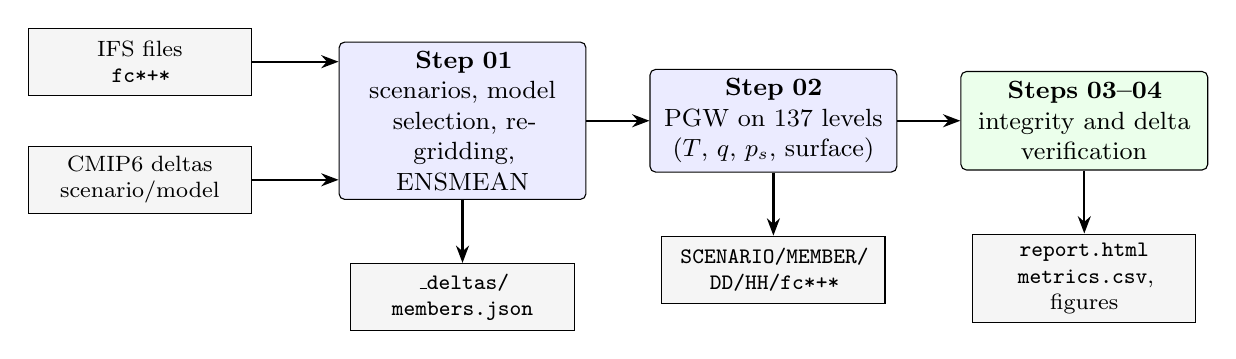
\begin{tikzpicture}[
  box/.style={draw, rounded corners=2pt, align=center, font=\small,
              minimum height=1.25cm, text width=2.9cm, fill=#1},
  box/.default=white,
  data/.style={draw, align=center, font=\footnotesize, minimum height=0.85cm,
               text width=2.6cm, fill=gray!8},
  arr/.style={-{Stealth[length=2.2mm]}, thick}]
  \node[box=blue!8] (s1) at (0,0)
    {\textbf{Step 01}\\scenarios, model\\selection, regridding,\\ENSMEAN};
  \node[box=blue!8, right=0.8cm of s1] (s2)
    {\textbf{Step 02}\\PGW on 137 levels\\($T$, $q$, $p_s$, surface)};
  \node[box=green!8, right=0.8cm of s2] (s3)
    {\textbf{Steps 03--04}\\integrity and delta\\verification};
  \node[data, left=1.1cm of s1, yshift=0.75cm] (ifs) {IFS files\\\code{fc*+*}};
  \node[data, left=1.1cm of s1, yshift=-0.75cm] (cmip) {CMIP6 deltas\\scenario/model};
  \node[data, below=0.8cm of s1] (dl) {\code{\_deltas/}\\\code{members.json}};
  \node[data, below=0.8cm of s2] (out) {\code{SCENARIO/MEMBER/}\\\code{DD/HH/fc*+*}};
  \node[data, below=0.8cm of s3] (rep) {\code{report.html}\\\code{metrics.csv}, figures};
  \draw[arr] (ifs.east) -- (s1.west |- ifs.east);
  \draw[arr] (cmip.east) -- (s1.west |- cmip.east);
  \draw[arr] (s1) -- (s2);
  \draw[arr] (s2) -- (s3);
  \draw[arr] (s1) -- (dl);
  \draw[arr] (s2) -- (out);
  \draw[arr] (s3) -- (rep);
\end{tikzpicture}
\caption{Structure of the workflow. Each scenario produces $X+1$ members
($X$ CMIP6 models and their ENSMEAN), and each member is a complete set of
HARMONIE boundary files.}
\label{fig:workflow}
\end{figure}

% ══════════════════════════════════════════════════════════════════════════════
\section{Step 01: scenarios, models and deltas on the HARMONIE grid}
\label{sec:step01}

\subsection{Scenario resolution}

Each scenario is a path under the delta root (\code{Future\_ssp585},
\code{Attribution/ssp245}, or equivalently \code{Attribution\_ssp245}). When
the scenario directory contains year subdirectories, the event year is taken
from the validity times of the IFS files, or from \code{ATTRIB\_YEAR} if the
user sets it. If the files span several years, the most frequent year is used
and a warning is printed.

\subsection{Model screening}

A model is a candidate when all required variables are present (\cref{tab:vars};
\code{ps} is added with \code{PS\_MODE=gcm} and \code{ua}, \code{va} with
\code{PERTURB\_WIND=true}). With \code{COMMON\_MODELS=true}, only models that
are complete in all requested scenarios are kept, so that differences between
scenarios do not arise from different model subsets. Models that fail any
check, or fail later while being read or regridded, are excluded with a
warning and the workflow continues. Exclusions and their reasons are written
to the log, to \code{\_deltas/members.json} and to the report. For the
combination of \code{Attribution\_ssp245} (2026) and \code{Future\_ssp585},
30 common models remain. Most exclusions arise from the absence of
\code{hurs} (for example, AWI-CM-1-1-MR, BCC-CSM2-MR, CAMS-CSM1-0, CIESM and
E3SM-1-0).

\subsection{Model selection}
\label{sec:selection}

The user chooses the models in one of three ways: an explicit list
(\code{MODELS="EC-Earth3 MIROC6 ..."}, case-insensitive), all candidates
(\code{MODELS=all}), or an automatic selection of $N$ models
(\code{MODELS=auto}, \code{N\_MODELS=N}).

The automatic selection describes each model $m$ with three domain features
computed on its native grid, inside the latitude--longitude box of the
HARMONIE domain (with a \ang{1} margin and $\cos\varphi$ area weights), and
averaged with the monthly weights of all the files to be perturbed:
\begin{equation}
  \mathbf{x}_m = \bigl(\, \overline{\dT}_{850-300},\ \Delta T_{\mathrm{as}},\
  \overline{\dRH}_{850-500} \,\bigr),
\end{equation}
where the overbars denote averages over the pressure levels between 850 and
\SI{300}{hPa} for temperature and between 850 and \SI{500}{hPa} for relative
humidity. Computing the features on the native grids avoids interpolating
the roughly 40 candidate models, and only the selected models are regridded.
With several scenarios and common models, the feature vectors of all
scenarios are concatenated. The features are standardized across the
candidates,
\begin{equation}
  z_{m,j} = \frac{x_{m,j} - \mu_j}{\sigma_j},
\end{equation}
and the distance of each model to the multi-model mean is
$d_m = \lVert \mathbf{z}_m \rVert$. Two methods are available:
\begin{description}
  \item[\code{spread} (default)] The first model is the one closest to the
    multi-model mean, $s_1 = \arg\min_m d_m$. Each additional model maximizes
    the minimum distance to the models already selected (farthest-point
    sampling),
    \begin{equation}
      s_{n+1} = \arg\max_{m \notin S_n}\ \min_{s \in S_n} \lVert \mathbf{z}_m - \mathbf{z}_s \rVert .
    \end{equation}
    The $N$ members therefore span the range of the full ensemble in the
    feature space. Their mean does not need to coincide with the mean of all
    candidates.
  \item[\code{representative}] The $N$ models with the smallest $d_m$.
\end{description}
The features of all candidates, the $z$-scores and the selected models are
stored in \code{members.json} and displayed in the report
(\cref{fig:selection}).

\subsection{Horizontal interpolation}

The deltas of each selected model are interpolated bilinearly from the GCM
grid to the geographical coordinates of every HARMONIE grid point, after
cropping a box around the domain with a \ang{3} margin and handling the
periodicity in longitude. Missing values below the GCM orography, or in
empty upper levels of some models, are filled beforehand by constant
vertical extrapolation from the nearest valid level. If the GRIB winds are
grid-relative, the $\Delta u$ and $\Delta v$ deltas are rotated to the
rotated-grid basis. The rotation angle is computed numerically from the
rotated-pole transform and ranges between \ang{-6.8} and \ang{6.8} in the
test domain.

\subsection{Ensemble mean}

For each scenario with at least two selected models, the ENSMEAN deltas are
the equal-weight mean of the regridded deltas of the $X$ models,
\begin{equation}
  \Delta_{\mathrm{ENS}} = \frac{1}{X}\sum_{m=1}^{X} \Delta_m ,
\end{equation}
for every month, level and variable. The intermodel standard deviation is
stored as \code{<var>\_spread}. The ENSMEAN is applied as one more member
(\cref{sec:step02}). Its perturbation is therefore internally consistent
(temperature, humidity and adjusted surface pressure are derived together)
and is not the average of the $X$ perturbed states.

% ══════════════════════════════════════════════════════════════════════════════
\section{Step 02: PGW on hybrid model levels}
\label{sec:step02}

The algorithm adapts \code{step\_03\_apply\_to\_era.py} of PGW4ERA5
\citep{Brogli2023} with \code{i\_reinterp = 0}: the deltas are applied at the
original pressures of the model levels and the driving fields are never
reinterpolated in the vertical.

\subsection{Hybrid coordinate}

With the half-level coefficients $(a_{k+1/2}, b_{k+1/2})$, the half-level and
full-level pressures of level $k$ are \citep{ECMWF_IFS_III}
\begin{equation}
  p_{k+1/2} = a_{k+1/2} + b_{k+1/2}\, p_s, \qquad
  p_k = \tfrac{1}{2}\left(p_{k-1/2} + p_{k+1/2}\right).
\end{equation}

\subsection{Temporal selection of the delta}

With \code{month=1..12}, the delta of that month is used for every file. With
\code{month=auto}, the delta at validity time $t$ is a linear interpolation
between the two months whose central dates $t_m$ and $t_{m+1}$ bracket $t$,
\begin{equation}
  \Delta(t) = (1 - w)\,\Delta_m + w\,\Delta_{m+1}, \qquad
  w = \frac{t - t_m}{t_{m+1} - t_m},
\end{equation}
which avoids jumps at month boundaries in long simulations.

\subsection{Vertical interpolation and surface anchor}

The 3D deltas are interpolated linearly in $\ln p$ to the original full-level
pressures, with constant extrapolation above the highest and below the lowest
GCM level, giving $\Delta_{\mathrm{std}}(p)$. For $\dT$ and $\dRH$, a
continuous surface correction makes the lowest levels approach the surface
deltas $\Delta_{\mathrm{sfc}}$ ($\Delta T_{\mathrm{as}}$, $\Delta\mathrm{RH_s}$):
\begin{equation}
  \Delta(p) = \Delta_{\mathrm{std}}(p) + \bigl[\Delta_{\mathrm{sfc}} - \Delta_{\mathrm{std}}(p_s)\bigr]
  \max\!\left(0,\ 1 - \frac{p_s - p}{D}\right),
  \label{eq:anchor}
\end{equation}
with $D = \SI{100}{hPa}$ (\code{SFC\_BLEND\_DEPTH}). PGW4ERA5 inserts the
surface value at the historical GCM surface pressure, which these deltas do
not provide. \Cref{eq:anchor} anchors the correction at the IFS surface
pressure instead. An earlier formulation that discarded the GCM levels below
$p_s$ produced discontinuities when $p_s$ crossed a pressure level. The
linear blend removes them and neutralizes the below-ground GCM values over
orography.

\subsection{Temperature}

\begin{equation}
  T' = T + \dT(p).
\end{equation}

\subsection{Specific humidity}

Relative humidity is computed with respect to the IFS mixed-phase saturation
vapor pressure \citep{ECMWF_IFS_IV},
\begin{equation}
  e_s(T) = \alpha\, e_{s,w}(T) + (1-\alpha)\, e_{s,i}(T), \quad
  \alpha = \min\!\left[1, \max\!\left(0, \frac{T - T_{\mathrm{ice}}}{T_0 - T_{\mathrm{ice}}}\right)\right]^2,
\end{equation}
with $e_{s,w}$ and $e_{s,i}$ given by the Tetens formula over water and ice,
$T_0 = \SI{273.16}{K}$ and $T_{\mathrm{ice}} = \SI{250.16}{K}$. The
conversions between $q$ and RH,
\begin{equation}
  \mathrm{RH} = \frac{e}{e_s(T)}, \quad e = \frac{q\,p}{\varepsilon + (1-\varepsilon)q},
  \quad q = \frac{\varepsilon\, e}{p - (1-\varepsilon)e},
\end{equation}
with $\varepsilon = R_d/R_v$, are exactly invertible, so that zero deltas
reproduce the original $q$. The perturbed relative humidity is
\begin{equation}
  \mathrm{RH}' = \min\!\Bigl[\max\bigl(\mathrm{RH} + \dRH,\ f\,\mathrm{RH}\bigr),\ \max(\mathrm{RH}, 1)\Bigr],
\end{equation}
with $f = 0.5$ (\code{RH\_MIN\_FACTOR}). The lower bound prevents $q \le 0$
in very dry air, such as intrusions with RH of about 0.4\% and $\dRH$ of
about $-3$\%. The upper bound keeps the supersaturation with respect to ice
that the IFS allows. The new specific humidity is
\begin{equation}
  q' = q + w_q(p)\,\bigl[q(\mathrm{RH}', T', p') - q\bigr], \qquad
  w_q = \min\!\left[1, \max\!\left(0, \frac{\ln p - \ln p_{\mathrm{top}}}{\ln p_{\mathrm{bot}} - \ln p_{\mathrm{top}}}\right)\right],
\end{equation}
with $p_{\mathrm{bot}} = \SI{150}{hPa}$ and $p_{\mathrm{top}} = \SI{100}{hPa}$.
Above $p_{\mathrm{top}}$ the specific humidity is not modified. Without this
taper, keeping RH under the stratospheric $\dT$ of the GCM produced
relative changes in $q$ between $+50$\% and $+300$\% in the attribution
deltas. Stratospheric water vapor is not controlled by relative humidity, so
these changes have no physical basis.

\subsection{Surface pressure}

With \code{PS\_MODE=hydrostatic} (default, as in PGW4ERA5), the surface
pressure is adjusted so that the change in geopotential at the reference
level $p_{\mathrm{ref}} = \SI{300}{hPa}$ matches the GCM delta of
geopotential height. The geopotential is integrated upward from the
(unchanged) surface geopotential over the half levels,
\begin{equation}
  \Phi_{k-1/2} = \Phi_{k+1/2} + R_d\, T_{v,k} \ln\frac{p_{k+1/2}}{p_{k-1/2}}, \qquad
  T_v = T\left[1 + \left(\varepsilon^{-1} - 1\right) q\right],
\end{equation}
and interpolated linearly in $\ln p$ to $p_{\mathrm{ref}}$. At iteration $n$,
with $q'$ recomputed from $\mathrm{RH}'$, $T'$ and the pressures implied by
$p_s^{(n)}$,
\begin{align}
  E^{(n)} &= \bigl[\Phi'(p_{\mathrm{ref}}) - \Phi(p_{\mathrm{ref}})\bigr] - g\,\Delta z_g(p_{\mathrm{ref}}), \\
  p_s^{(n+1)} &= p_s^{(n)} - \lambda\, \frac{p_s^{(n)}}{R_d\, T'_L}\, E^{(n)},
\end{align}
where $T'_L$ is the perturbed temperature of the lowest model level and
$\lambda = 0.95$. The factor $p_s/(R_d T)$ is the inverse of the hydrostatic
sensitivity $\partial\Phi/\partial p_s$. The iteration stops when
$\max|E| < \SI{0.15}{m^2.s^{-2}}$ (about \SI{1.5}{cm}), with a maximum of 20
iterations. It converges in 6 iterations in the test case. The output field is
$\ln p_s'$. The alternatives \code{PS\_MODE=gcm} ($p_s + \Delta p_s$ of the
GCM) and \code{none} are available.

\subsection{Wind (optional)}

With \code{PERTURB\_WIND=true}, $u' = u + \Delta u$ and $v' = v + \Delta v$,
with the rotated deltas and without surface anchor, as in PGW4ERA5. The
default leaves the wind unchanged, so the default experiments perturb only
the thermodynamic state.

\subsection{Surface and soil}

The GCM \code{ts} delta mixes land and sea signals near the coast. Over the
sea, an open-sea delta is used: the sea mask ($\mathrm{lsm} < 0.5$) is
eroded by two grid points, the remaining points are filled by
inverse-distance weighting from the eight nearest open-sea points (weights
$d^{-2}$), and the result is smoothed with a Gaussian filter of one grid
point. The perturbations are
\begin{itemize}
  \item skin temperature: $\mathrm{skt}' = \mathrm{skt} + \Delta T_s$, with
    the open-sea delta over the sea and the GCM delta over land;
  \item sea surface temperature: $\mathrm{sst}' = \mathrm{sst} + \Delta T_s$
    at the valid points, keeping the bitmap;
  \item soil temperatures (layers centered at 0.035, 0.175, 0.64 and
    \SI{1.945}{m}), following PGW4ERA5:
    \begin{equation}
      \Delta T_{\mathrm{soil}}(z) = \overline{\Delta T_s} + e^{-z/z_e}\,\bigl(\Delta T_s - \overline{\Delta T_s}\bigr),
      \qquad z_e = \SI{2.8}{m},
    \end{equation}
    where $\overline{\Delta T_s}$ is the annual mean delta, so that the
    seasonal cycle of the delta is damped with depth.
\end{itemize}
Soil moisture, snow, sea ice, land--sea mask, surface geopotential and the
remaining surface fields are not modified.

\subsection{GRIB output}

All messages are written in their original order and with their original
metadata, and only the values of the perturbed fields are replaced. Each file
is written to a temporary name and renamed once complete. Members and files
are independent and are processed in a common pool of processes.

% ══════════════════════════════════════════════════════════════════════════════
\section{Steps 03 and 04: verification}
\label{sec:verif}

Step~03 checks the integrity of each member: number of messages, metadata
(parameter, level, date, step, grid, packing), bit-identical values of every
non-perturbed field, finite values, $q \ge 0$ and an unchanged SST bitmap.

Step~04 checks that the deltas were applied correctly. For each scenario,
member and file, the expected change of each field is recomputed and compared
with the difference between the PGW and the original files. GRIB encoding
quantizes each value with a step
\begin{equation}
  u = 2^{E}\,10^{-D},
\end{equation}
where $E$ and $D$ are the binary and decimal scale factors of the message.
Errors of the exact replicas are expressed in these packing units (p.u.).
Rounding to the nearest representable value gives errors of at most
\SI{0.5}{p.u.} \Cref{tab:checks} summarizes the checks and tolerances.

\begin{table}[htbp]
\centering
\caption{Checks of Step~04. p.u.: GRIB packing units.}
\label{tab:checks}
\small
\begin{tabularx}{\linewidth}{lXl}
\toprule
Check & Comparison & Tolerance \\
\midrule
Replica of $T$, $q$, skt, sst, stl1--4 ($u$, $v$) & written change minus the
  change recomputed with the package formulas and the final $p_s$ of the file & $\le$ \SI{1}{p.u.} \\
$\dT$ on sample columns & 300 columns with an independent vertical
  interpolation (\code{numpy.interp}) & $\le$ \SI{e-3}{K} + packing \\
$\Delta z_g(p_{\mathrm{ref}})$ & $[\Phi'(p_{\mathrm{ref}}) - \Phi(p_{\mathrm{ref}})]/g$
  minus the GCM $\Delta z_g$ & max $\le$ \SI{0.25}{m} \\
$\dRH$ in the troposphere & RH recomputed from the final $T$, $q$, $p$ minus
  $\mathrm{RH} + \dRH$, at $p \ge p_{\mathrm{bot}}$ and outside the bounded points & RMSE $\le$ 0.5\% \\
Stratospheric $q$ & change of $q$ above $p_{\mathrm{top}}$ & $\le$ \SI{1}{p.u.} \\
SST bitmap, $q \ge 0$ & & exact \\
Regridding & deltas on the grid minus \code{xarray.interp} of the native
  deltas (300 points; tas, ta at \SI{500}{hPa}, ts) & $\le$ \SI{0.02}{K} \\
ENSMEAN deltas & ENSMEAN minus the mean of the model deltas & $\le 10^{-4}$ \\
ENSMEAN applied $\dT$ & $\dT$ of the ENSMEAN minus the mean $\dT$ of the
  models ($\dT$ is linear in $\Delta$) & $\le$ \SI{0.01}{K} \\
\bottomrule
\end{tabularx}
\end{table}

The ENSMEAN changes of RH and $p_s$ are also compared with the means of the
model changes, but only for information: the bounds on RH and the iterative
adjustment of $p_s$ are nonlinear in $\Delta$, so exact agreement is not
expected. The results are written to \code{verification/report.html} (a
self-contained HTML file with tables and figures), \code{metrics.csv} (one
row per scenario, member, file and check) and \code{summary.txt}. The job
exits with an error if any check fails, after running all steps.

% ══════════════════════════════════════════════════════════════════════════════
\section{Example: western Mediterranean, 4 October 2026}
\label{sec:example}

\subsection{Configuration}

The example perturbs the IFS analysis file valid at 00~UTC on 4 October 2026
for the HARMONIE domain \code{BCN\_Tropical} (\ang{33.8}--\ang{48.0}N,
\ang{7.7}W--\ang{13.0}E). The configuration uses the default options of
\cref{tab:opts} with \code{month=10}: the attribution scenario for the event
year 2026 (historical 1850--1879 minus 2011--2040) and the ssp585 projection
(2070--2099 minus 1985--2014), with $N = 5$ common models selected
automatically with the \code{spread} method. The test ran with four
processes. Each pair of member and file took between 4 and \SI{8}{s} in
Step~02.

\subsection{Model selection}

Of the 47 models in the attribution directory and 38 in the ssp585 directory,
30 are complete in both scenarios. The selection returns CMCC-CM2-SR5 (the
model closest to the multi-model mean), CanESM5, FIO-ESM-2-0, GISS-E2-2-G and
EC-Earth3-Veg. In the attribution scenario, these models range from the
strongest tropospheric cooling of the candidates (CanESM5, $-3.4$~K between
850 and \SI{300}{hPa}) to one of the weakest (GISS-E2-2-G, $-1.2$~K), and
from the largest decrease in relative humidity (FIO-ESM-2-0, $-1.8$\%) to an
increase of $+2.6$\% (\cref{fig:selection}). The mean of the five selected
models differs from the mean of the 30 candidates by $-0.18$~K in
tropospheric $\dT$ and by $-0.59$ percentage points in $\dRH$ in the
attribution scenario, and by $+0.18$~K and $+0.65$ percentage points in the
ssp585 scenario.

\begin{figure}[htbp]
\centering
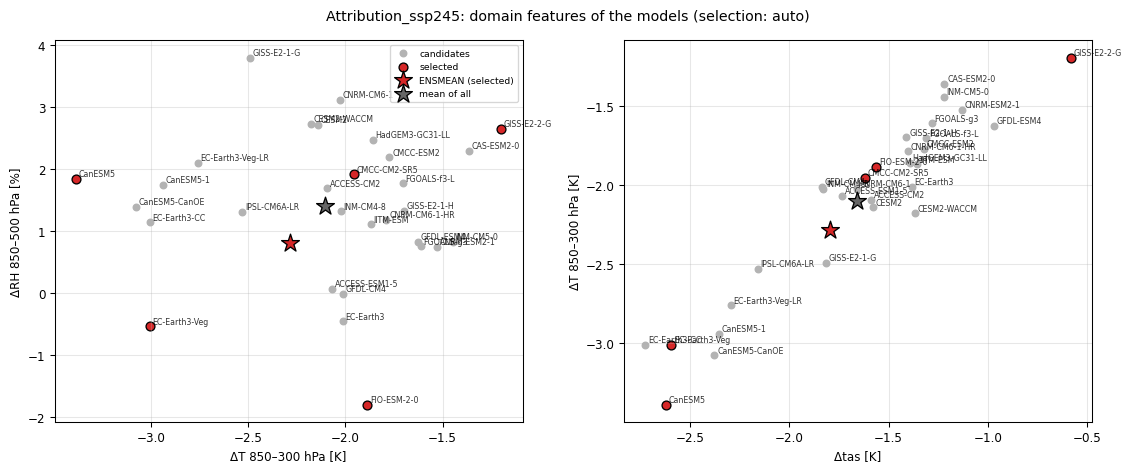
\includegraphics[width=\linewidth]{selection_Attribution_ssp245.png}
\caption{Domain features of the 30 candidate models in the attribution
scenario (2026): (left) mean $\dRH$ between 850 and \SI{500}{hPa} against
mean $\dT$ between 850 and \SI{300}{hPa}, and (right) mean $\dT$ between 850
and \SI{300}{hPa} against $\Delta T_{\mathrm{as}}$. Gray dots are the
candidates, red dots the five models selected with the \code{spread} method
on the concatenated features of the attribution and ssp585 scenarios, the red
star the mean of the selected models (ENSMEAN) and the gray star the mean of
all candidates.}
\label{fig:selection}
\end{figure}

\subsection{Applied perturbation}

\Cref{tab:example} lists the domain means of the applied changes for each
member. In the attribution scenario, the ENSMEAN cools the domain by
\SI{2.00}{K} at \SI{850}{hPa} and by \SI{2.38}{K} at \SI{500}{hPa}, and the
five models span from $-1.08$ to \SI{-3.02}{K} at \SI{850}{hPa}. In the
ssp585 scenario, the ENSMEAN warms the domain by \SI{5.25}{K} at
\SI{850}{hPa} and \SI{6.04}{K} at \SI{500}{hPa}, with model values between
$+3.34$ and \SI{+7.58}{K} at \SI{850}{hPa}. The intermodel standard deviation
of $\dT$ at the lowest model level ranges between 0.60 and \SI{1.06}{K}
across the domain in the attribution scenario and between 0.96 and
\SI{1.71}{K} in the ssp585 scenario (\cref{fig:maps}).

Specific humidity at \SI{850}{hPa} decreases by 11.5\% in the attribution
ENSMEAN and increases by 32.9\% in the ssp585 ENSMEAN, which corresponds to
5.8 and 6.3\% per kelvin of the local $\dT$. These rates combine the
temperature dependence of the saturation vapor pressure (about 7\%~K$^{-1}$
near the surface) with the imposed $\dRH$ of $+0.48$ and $-2.90$ percentage
points. Above \SI{100}{hPa} the specific humidity is unchanged by
construction, while $\dT$ changes sign: stratospheric cooling in ssp585 and
warming in the attribution deltas (\cref{fig:scenarios}). The surface
pressure adjustment converged in five or six iterations for every member.
The domain-mean $\Delta p_s$ ranges from $-110$ to \SI{+225}{Pa} across
members, with the largest positive values over the main mountain ranges of
the domain.

\begin{table}[htbp]
\centering
\caption{Domain-mean applied changes for each member (file valid at 00~UTC
on 4 October 2026). $\dT$ and $\dRH$ are evaluated at the model level closest
to each pressure level. $\Delta$SST is the mean over valid sea points.}
\label{tab:example}
\small
\begin{tabular}{llrrrrr}
\toprule
Scenario & Member & $\dT_{850}$ (K) & $\dT_{500}$ (K) & $\dRH_{850}$ (\%) & $\Delta p_s$ (Pa) & $\Delta$SST (K) \\
\midrule
Attribution (2026) & CMCC-CM2-SR5  & $-1.63$ & $-2.04$ & $+0.58$ & $-105.7$ & $-1.30$ \\
                   & CanESM5       & $-3.02$ & $-3.51$ & $+1.01$ & $-94.9$  & $-2.33$ \\
                   & FIO-ESM-2-0   & $-1.61$ & $-1.98$ & $-1.68$ & $+134.4$ & $-1.28$ \\
                   & GISS-E2-2-G   & $-1.08$ & $-1.20$ & $+3.59$ & $-44.2$  & $-0.14$ \\
                   & EC-Earth3-Veg & $-2.69$ & $-3.16$ & $-1.21$ & $+152.5$ & $-2.20$ \\
                   & \textbf{ENSMEAN} & $\mathbf{-2.00}$ & $\mathbf{-2.38}$ & $\mathbf{+0.48}$ & $\mathbf{+8.6}$ & $\mathbf{-1.45}$ \\
\midrule
ssp585             & CMCC-CM2-SR5  & $+5.45$ & $+6.09$ & $-3.40$ & $-37.6$  & $+4.04$ \\
                   & CanESM5       & $+7.58$ & $+8.42$ & $-3.87$ & $+71.8$  & $+6.30$ \\
                   & FIO-ESM-2-0   & $+4.69$ & $+5.14$ & $-5.14$ & $+77.0$  & $+3.48$ \\
                   & GISS-E2-2-G   & $+3.34$ & $+4.12$ & $-1.28$ & $-109.6$ & $+2.92$ \\
                   & EC-Earth3-Veg & $+5.16$ & $+6.44$ & $-0.83$ & $+225.3$ & $+4.37$ \\
                   & \textbf{ENSMEAN} & $\mathbf{+5.25}$ & $\mathbf{+6.04}$ & $\mathbf{-2.90}$ & $\mathbf{+46.7}$ & $\mathbf{+4.22}$ \\
\bottomrule
\end{tabular}
\end{table}

\begin{figure}[htbp]
\centering
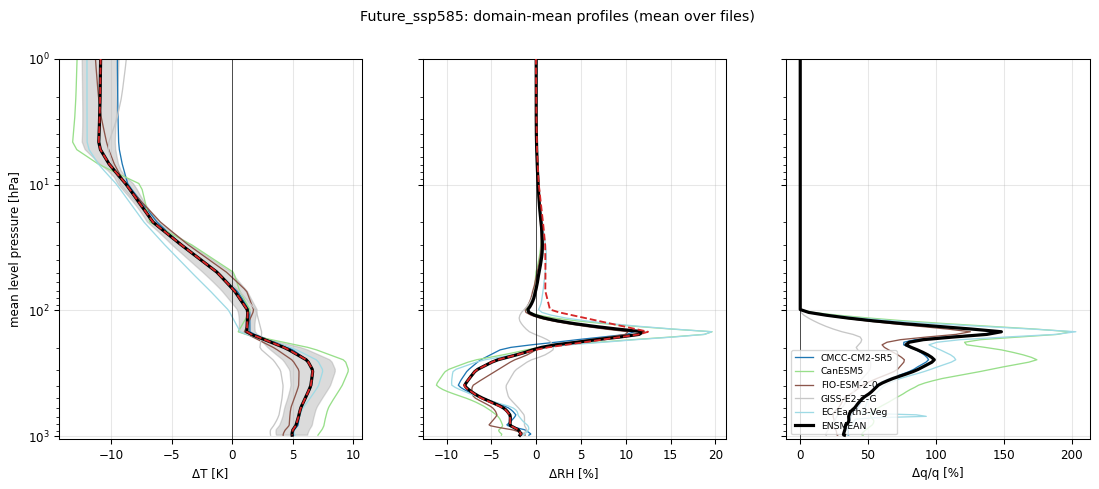
\includegraphics[width=\linewidth]{profiles_Future_ssp585.png}
\caption{Domain-mean profiles of the applied changes in the ssp585 scenario:
(left) $\dT$, (center) $\dRH$ and (right) relative change in specific
humidity, against the mean pressure of each model level. Thin colored lines
are the five models, the thick black line is the ENSMEAN and the gray band is
$\pm1$ intermodel standard deviation of $\dT$. Dashed red lines are the
expected $\dT$ and the unbounded target $\dRH$ of the ENSMEAN. The target and
reached $\dRH$ differ above \SI{150}{hPa} because of the stratospheric taper
of $\Delta q$.}
\label{fig:profiles}
\end{figure}

\begin{figure}[htbp]
\centering
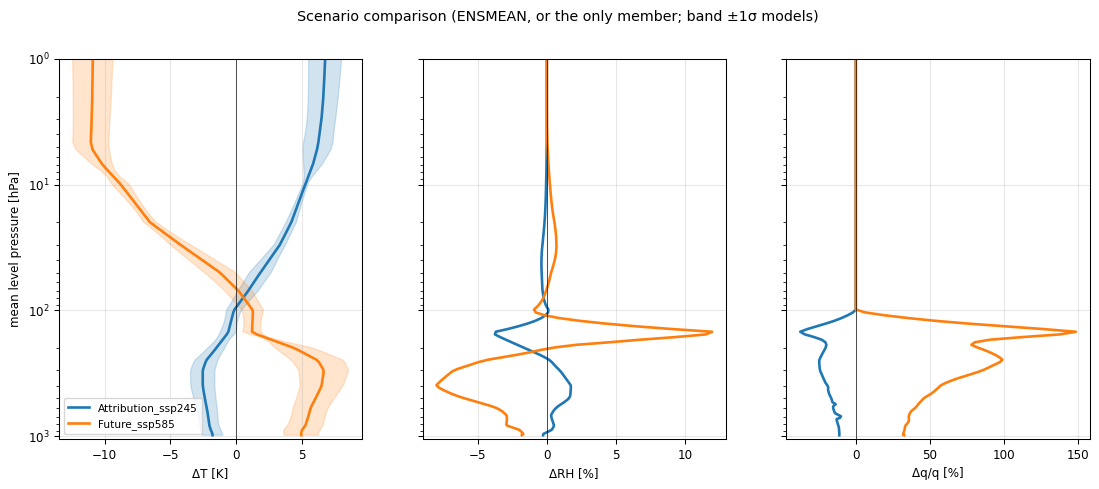
\includegraphics[width=0.85\linewidth]{scenarios.png}
\caption{ENSMEAN profiles of (left) $\dT$, (center) $\dRH$ and (right)
relative change in specific humidity for the attribution (blue) and ssp585
(orange) scenarios. Shading shows $\pm1$ intermodel standard deviation of
$\dT$.}
\label{fig:scenarios}
\end{figure}

\begin{figure}[htbp]
\centering
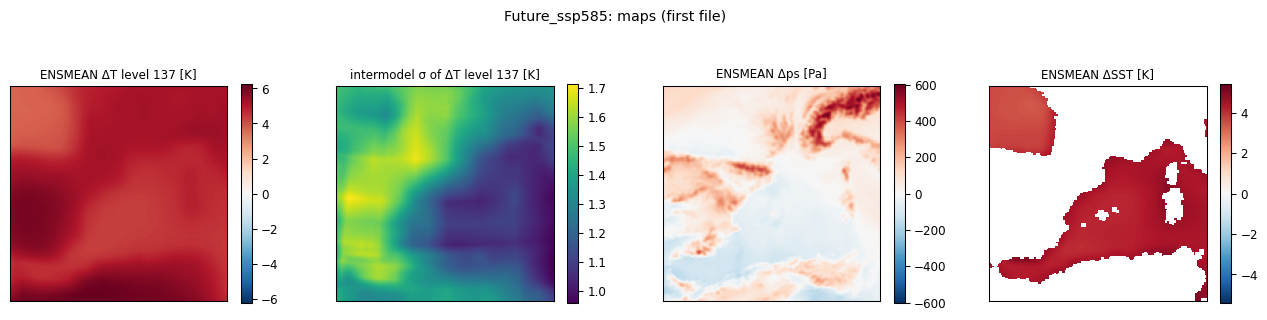
\includegraphics[width=\linewidth]{maps_Future_ssp585.png}
\caption{Maps for the ssp585 scenario: (from left to right) ENSMEAN $\dT$ at
the lowest model level, intermodel standard deviation of $\dT$ at the lowest
model level, ENSMEAN $\Delta p_s$ and ENSMEAN $\Delta$SST (land points
masked). Axes are the rotated-grid indices.}
\label{fig:maps}
\end{figure}

\subsection{Verification}

All checks of \cref{tab:checks} pass for the 12 members (\cref{fig:errors}).
The exact replicas of $T$, skt, sst and stl1--4 have maximum errors of
\SI{0.50}{p.u.}, the rounding limit of the encoding, which corresponds to
\SI{2.4e-4}{K} for $T$. The replica of $q$ reaches \SI{0.77}{p.u.}, because
the expected $q$ is recomputed with the surface pressure decoded from the
PGW file. The independent interpolation on 300 columns agrees with the
applied $\dT$ within \SI{2.4e-4}{K}. The geopotential height change at
\SI{300}{hPa} departs from the GCM target by at most \SI{3.7}{cm} (RMSE of
\SI{1.7}{cm} in the worst member). The reached $\dRH$ in the troposphere
departs from the target by an RMSE of 0.001\%. The specific humidity above
\SI{100}{hPa} is bit-identical to the original. The regridded deltas agree
with \code{xarray.interp} of the native fields within \SI{5e-7}{K}, and the
ENSMEAN deltas equal the mean of the five models within the float32
precision. The applied $\dT$ of the ENSMEAN equals the mean of the applied
$\dT$ of the models within \SI{4.6e-4}{K}. The ENSMEAN changes of RH and
$p_s$ differ from the means of the model changes by up to 2.6 percentage
points and \SI{3.8}{Pa}, respectively, which reflects the nonlinearity of the
RH bounds and of the surface pressure adjustment.

\begin{figure}[htbp]
\centering
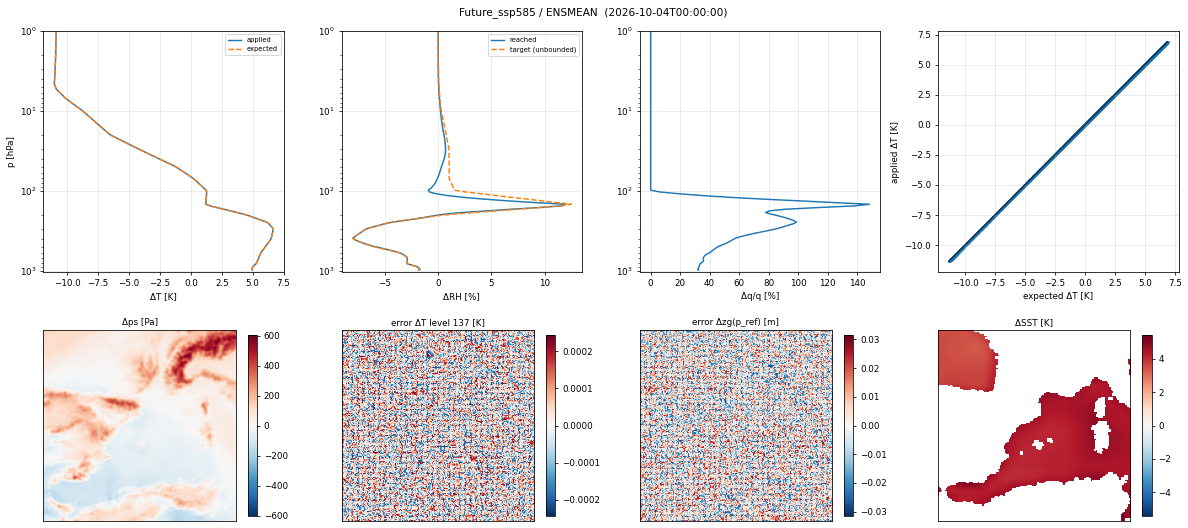
\includegraphics[width=\linewidth]{member_Future_ssp585_ENSMEAN.png}
\caption{Verification of the ssp585 ENSMEAN member. Top row: domain-mean
applied and expected $\dT$, reached and target $\dRH$, relative change in
specific humidity, and applied against expected $\dT$ on 300 columns and
137 levels. Bottom row: $\Delta p_s$, error of $\dT$ at the lowest model
level, error of $\Delta z_g$ at \SI{300}{hPa}, and $\Delta$SST. The error
maps show the white noise of the GRIB quantization.}
\label{fig:member}
\end{figure}

\begin{figure}[htbp]
\centering
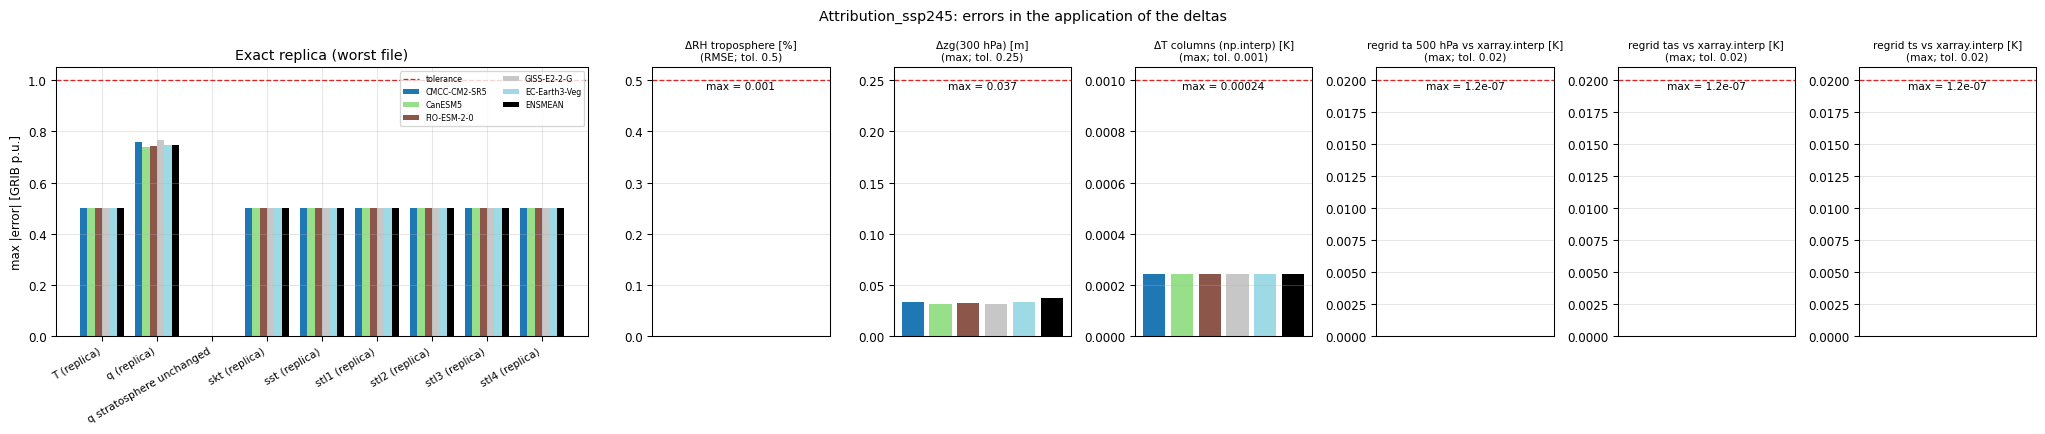
\includegraphics[width=\linewidth]{errors_Attribution_ssp245.png}
\caption{Worst error per member and check in the attribution scenario.
Left: exact replicas in GRIB packing units. Right panels: physical and
independent checks in their own units. Dashed red lines mark the tolerances
of \cref{tab:checks}.}
\label{fig:errors}
\end{figure}

\clearpage

% ══════════════════════════════════════════════════════════════════════════════
\section{Usage}
\label{sec:usage}

\subsection{Software environment}

The tested environment is loaded with \code{source env.sh}
(ecmwf-toolbox 2026.04 with the HARMONIE ecCodes definitions, ecCodes 2.47,
and python3/3.11.10-01 with xarray, scipy, eccodes and matplotlib). Other
module combinations can fail when decoding the CCSDS-packed specific
humidity.

\subsection{Running the workflow}

The options are set at the top of \code{run\_PGW\_HARMONIE\_ML.sh}
(\cref{tab:opts}), and the job is submitted with
\begin{lstlisting}[language=bash]
sbatch run_PGW_HARMONIE_ML.sh <path_input> <path_output> <cmip_root> <month>

# example
sbatch run_PGW_HARMONIE_ML.sh \
    /ec/res4/scratch/spcc/hm_home/ECMWF/BCN_Tropical/2026/10 \
    /ec/res4/scratch/ecme2143/PGW_BCN_Tropical/2026/10 \
    /ec/res4/hpcperm/ecme2143/CMIP6_deltas 10
\end{lstlisting}
The script can be submitted from any directory. The code is taken from the
physical location of the script, and relative paths are resolved with respect
to the submission directory. The SLURM log is written to \code{logs/} relative
to the submission directory. The output tree is
\begin{lstlisting}
<path_output>/
  _deltas/members.json, members.txt
  _deltas/<SCENARIO>/<MODEL|ENSMEAN>/deltas_on_grid.nc
  <SCENARIO>/<MEMBER>/DD/HH/fcYYYYMMDD_HH+000     (PGW files)
  <SCENARIO>/<MEMBER>/pgw_options.json, pgw_diagnostics.jsonl
  verification/report.html, metrics.csv, summary.txt, figs/
\end{lstlisting}
A HARMONIE experiment uses one member by pointing its boundary directory
(\code{BDDIR}) to the directory of that member,
\code{<path\_output>/<SCENARIO>/} \code{<MEMBER>}.

\begin{table}[htbp]
\centering
\caption{Main options of \code{run\_PGW\_HARMONIE\_ML.sh}.}
\label{tab:opts}
\small
\begin{tabularx}{\linewidth}{>{\raggedright\arraybackslash}p{4.6cm}>{\raggedright\arraybackslash}p{3.6cm}X}
\toprule
Option & Default & Meaning \\
\midrule
\code{SCENARIOS} & \code{Attribution\_ssp245} \code{Future\_ssp585} & scenarios under \code{cmip\_root}, or \code{all} \\
\code{ATTRIB\_YEAR} & \code{auto} & event year of the attribution deltas \\
\code{MODELS} & \code{auto} & explicit list, \code{all} or \code{auto} \\
\code{N\_MODELS} & 5 & number of models with \code{auto} \\
\code{AUTO\_METHOD} & \code{spread} & \code{spread} or \code{representative} \\
\code{COMMON\_MODELS} & \code{true} & same models in all scenarios \\
\code{MAKE\_ENSMEAN} & \code{true} & additional ENSMEAN member \\
\midrule
\code{PERTURB\_T}, \code{PERTURB\_Q} & \code{true} & temperature and humidity \\
\code{PERTURB\_WIND} & \code{false} & $u$, $v$ \\
\code{PS\_MODE} & \code{hydrostatic} & \code{hydrostatic}, \code{gcm} or \code{none} \\
\code{P\_REF} & \SI{30000}{Pa} & reference level of the $p_s$ adjustment \\
\code{SFC\_ANCHOR}, \code{SFC\_BLEND\_DEPTH} & \code{true}, \SI{10000}{Pa} & surface anchor of $\dT$, $\dRH$ \\
\code{Q\_TAPER\_BOTTOM/TOP} & 15000/\SI{10000}{Pa} & stratospheric taper of $\Delta q$ \\
\code{RH\_MIN\_FACTOR} & 0.5 & lower bound of $\mathrm{RH}'$ \\
\code{PERTURB\_SKT/SST/SOIL} & \code{true} & surface and soil \\
\code{COAST\_BUFFER}, \code{SST\_SMOOTH\_SIGMA} & 2, 1.0 & open-sea $\Delta T_s$ \\
\bottomrule
\end{tabularx}
\end{table}

% ══════════════════════════════════════════════════════════════════════════════
\section{Limitations}
\label{sec:limits}

\begin{itemize}
  \item The experiments keep the synoptic evolution of the driving analysis.
    They evaluate conditional changes in the simulated event and do not
    estimate changes in its probability, frequency or circulation.
  \item The wind is not perturbed by default. Similar winds in the
    perturbed simulations therefore reflect the design and cannot be
    interpreted as an absence of dynamical change under the imposed
    climate state.
  \item The deltas are monthly climatological differences. Sub-monthly
    variability of the climate signal and its dependence on the weather
    regime are not represented.
  \item The $X$ selected models sample part of the intermodel uncertainty of
    $\Delta$. With \code{AUTO\_METHOD=spread}, the selection spans the range
    of three domain-mean features, and the ENSMEAN of the $X$ models can
    differ from the mean of all candidates (\cref{fig:selection}). Internal
    variability within each model and uncertainty in the construction of the
    perturbation are not sampled.
  \item Constant extrapolation is used above the highest GCM level
    (\SI{1}{hPa}) and below the lowest one. The specific humidity is not
    perturbed above \SI{100}{hPa}.
  \item The integration of HARMONIE with the perturbed files (boundary
    processing and forecast) has not been tested yet.
\end{itemize}

% ══════════════════════════════════════════════════════════════════════════════
\section*{Code availability}
The workflow is written in Python (numpy, scipy, xarray, eccodes, matplotlib)
and Bash. The repository includes a round-trip test
(\code{tests/test\_zero\_deltas.py}) that applies zero deltas and checks that
the output reproduces the input within one packing unit.

\begin{thebibliography}{9}
\bibitem[Brogli et al.(2023)]{Brogli2023}
Brogli, R., Heim, C., Mensch, J., S{\o}rland, S.~L., and Sch{\"a}r, C.:
The pseudo-global-warming (PGW) approach: methodology, software package
PGW4ERA5 v1.1, validation, and sensitivity analyses, Geosci. Model Dev., 16,
907--926, \url{https://doi.org/10.5194/gmd-16-907-2023}, 2023.

\bibitem[ECMWF(a)]{ECMWF_IFS_III}
ECMWF: IFS Documentation, Part III: Dynamics and Numerical Procedures,
European Centre for Medium-Range Weather Forecasts, Reading, UK.

\bibitem[ECMWF(b)]{ECMWF_IFS_IV}
ECMWF: IFS Documentation, Part IV: Physical Processes, European Centre for
Medium-Range Weather Forecasts, Reading, UK.

\bibitem[Eyring et al.(2016)]{Eyring2016}
Eyring, V., Bony, S., Meehl, G.~A., Senior, C.~A., Stevens, B., Stouffer,
R.~J., and Taylor, K.~E.: Overview of the Coupled Model Intercomparison
Project Phase 6 (CMIP6) experimental design and organization, Geosci. Model
Dev., 9, 1937--1958, \url{https://doi.org/10.5194/gmd-9-1937-2016}, 2016.

\bibitem[Sch{\"a}r et al.(1996)]{Schar1996}
Sch{\"a}r, C., Frei, C., L{\"u}thi, D., and Davies, H.~C.: Surrogate
climate-change scenarios for regional climate models, Geophys. Res. Lett.,
23, 669--672, \url{https://doi.org/10.1029/96GL00265}, 1996.
\end{thebibliography}

\end{document}
